% =========================
% Project Documentation
% =========================

\section{Project documentatie}
\label{sec:project-documentatie}

\subsection{Inleiding}
\label{sec:project-documentatie-inleiding}

In dit hoofdstuk wordt er gekeken naar hoe de individuele samenvattingen van een Python bestand gebruikt kunnen worden om een samenvatting van het gehele project te maken.
Alsook wordt er verder gekeken naar hoe de relaties tussen de verschillende bestanden gevisualiseerd kunnen worden.
Dit om een zo goed mogelijk overzicht te krijgen van het project, zonder dat er handmatig documentatie moet worden geschreven.

\subsection{Projectsamenvatting}
\label{sec:project-documentatie-samenvatting}

De samenvatting van een Python project kan gemaakt worden door de individuele samenvattingen van de bestanden samen te voegen.
Deze samenvatting kan bekomen worden door elk python bestand in het project te laten documenteren en de samenvatting ervan op te slaan.
Erna kunnen deze samenvattingen samengevoegd worden om dan mee te geven aan een Large Language Model.
Deze samenvattingen worden gegenereerd door het aanroepen van de functie \mintinline{python3}|generate_file_summaries()|. 
Deze functie maakt gebruik van de klasse \mintinline{python3}|FileDocumenationGenerator()| die de samenvattingen van de bestanden genereerd en opslaat in een dictionary.
De code van deze functie is te vinden in \ref{bijlage:file-summary-functions}.  

Door een duidelijk prompt mee te geven aan het model, kan er specifiek gevraagd worden welke functies en klassen er in het project zitten en dat per bestand duidelijk opgelijst. Samen met deze oplijsting wordt er ook een korte samenvatting van het gehele project weergegeven.
Een voorbeeld van de uitkomst is te zien in \ref{fig:project-summary}.
Hier is te zien dat er een duidelijk overzicht is van welke functies en klassen er in het project zitten, alsook wat het gehele project inhoudt.

\begin{figure}[h]
    \centering
    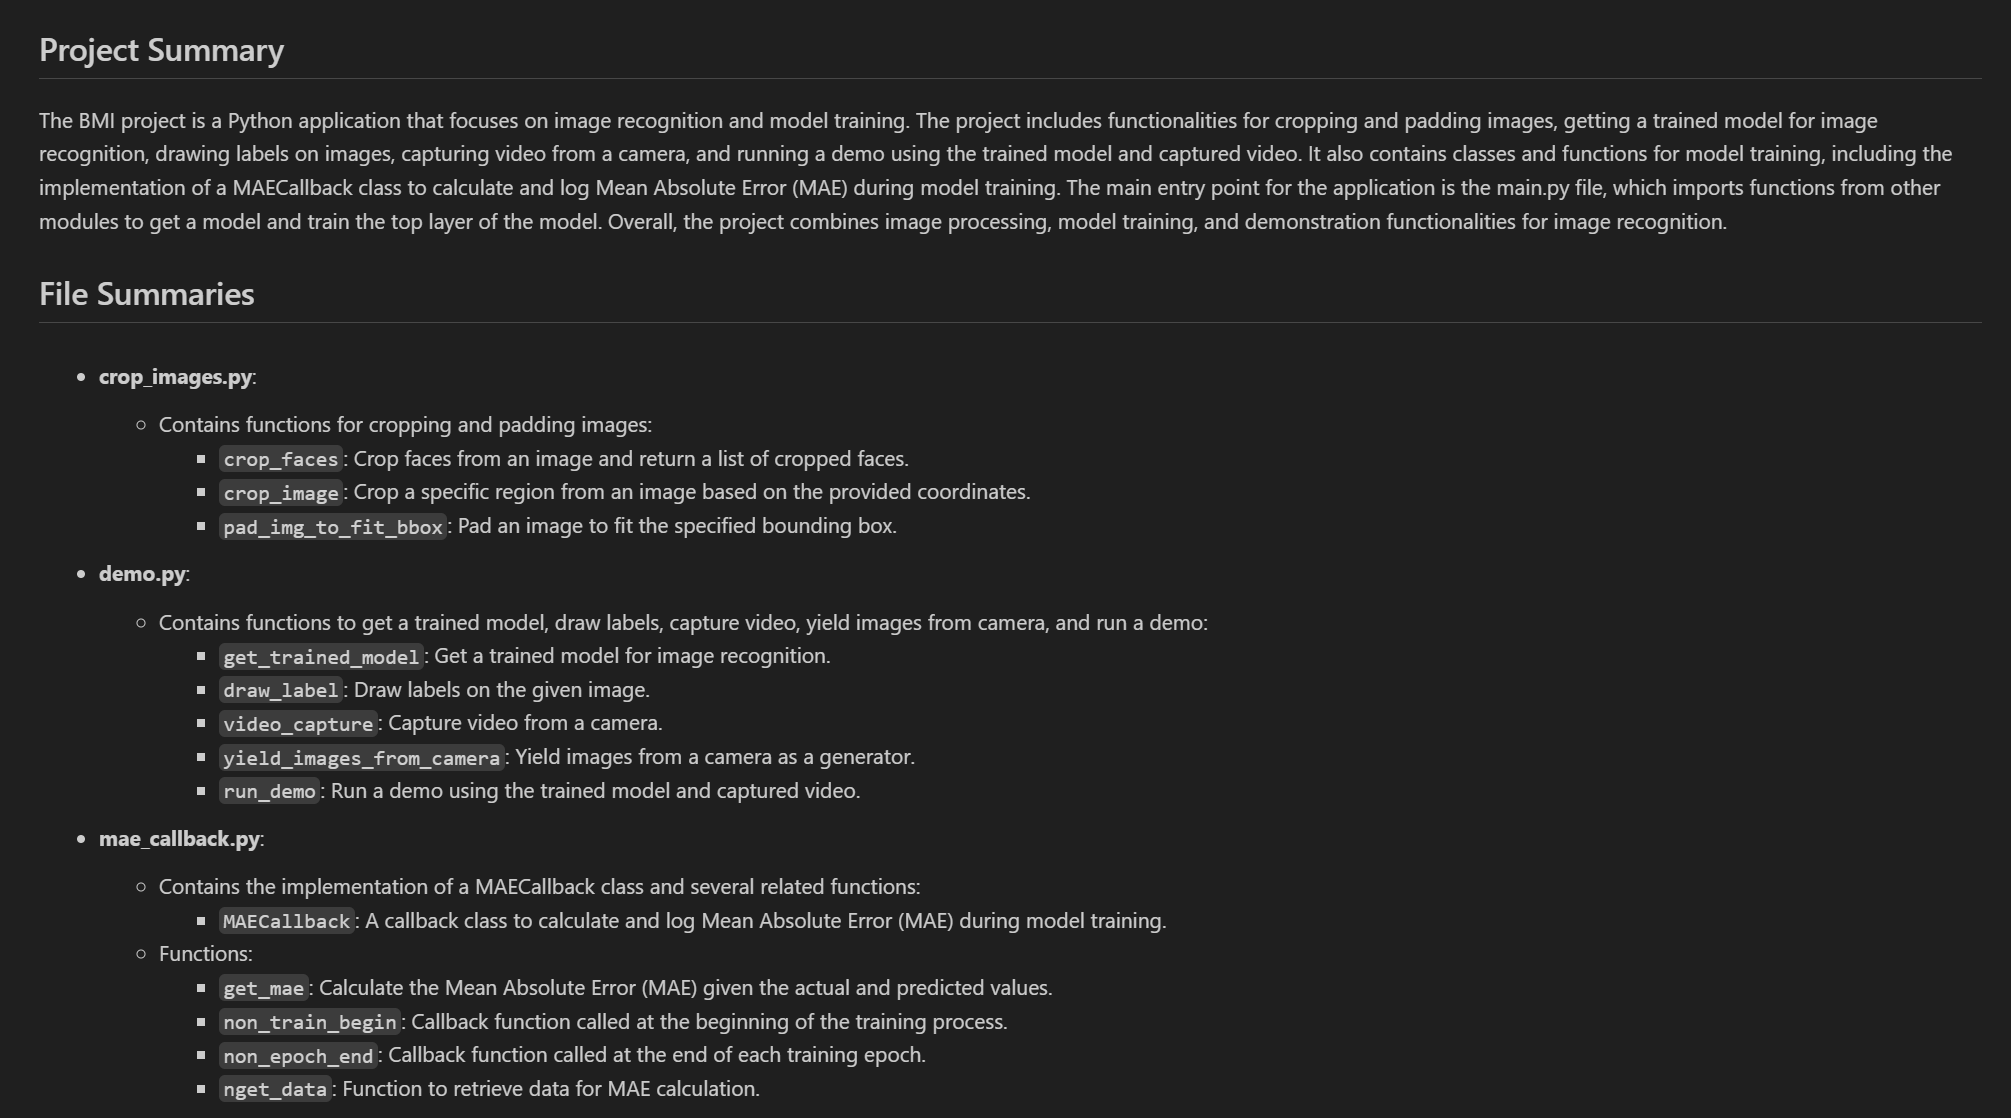
\includegraphics[width=1\textwidth]{project_summary.png}
    \caption{Voorbeeld van een project samenvatting}
    \label{fig:project-summary}
\end{figure}    

\subsubsection{Keuze van welke bestanden te documenteren}
\label{subsec:project-documentatie-keuze-bestanden}

Het is belangrijk om te kijken naar welke bestanden er gedocumenteerd moeten worden.
Omdat het gaat over een Python project, is het belangrijk dat alle Python bestanden gedocumenteerd worden.
Er is de keuze gemaakt om het bestand \mintinline{python3}|__init__.py| niet te documenteren, omdat dit bestand vaak niet relevant is voor de documentatie van het project.
Dit omdat het bestand vaak leeg is of slechts minimale functionaliteit bevat. 
Ook bevat het soms enkele configuratie opties die niet relevant zijn voor de documentatie.

\subsubsection{Documentatie van bestanden zonder functies of klassen}
\label{subsec:project-documentatie-geen-functies}

Omdat er eerst vanuit gegaan wordt dat elk bestand functies of klassen bevat, is het belangrijk om te kijken naar bestanden die dit niet bevatten.
Deze bestanden dienen ook gedocumenteerd te worden om een volledig overzicht te krijgen van het project.
Als er geen apart prompt voorzien wordt dan zal het model hallucineren en een samenvatting verzinnen, dit is niet de bedoeling.
Er is gebruik gemaakt van een prompt \ref{bijlage:bestand-zonder-functies} die vraagt om de werking van het document uit te leggen en de eventuele imports die het bestand bevat.
In dit prompt wordt er duidelijk gedefinieerd wat er in de documentatie moet staan. 
En aan de hand van een voorbeeld wordt er getoond hoe de documentatie eruit moet zien.
Een voorbeeld van de uitkomst in de project documentatie van een bestand zonder functies is te zien in \ref{fig:file-no-functions}.

\begin{figure}[h]
    \centering
    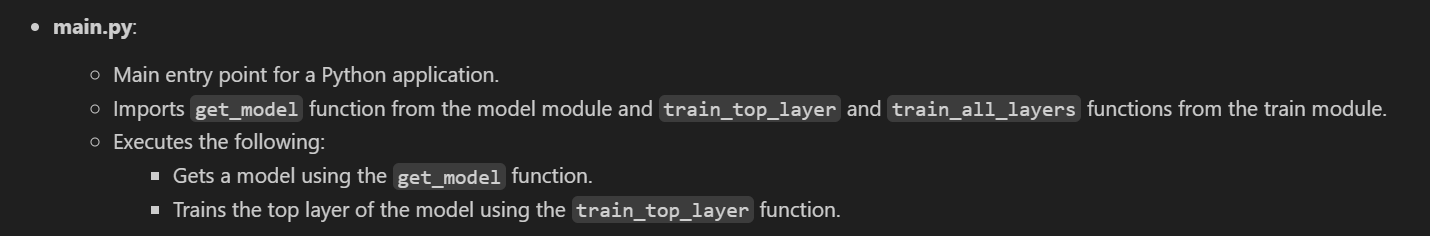
\includegraphics[width=1\textwidth]{documentatie_bestand_zonder_functies.png}
    \caption{Voorbeeld van de documentatie van een bestand zonder functies of klassen}
    \label{fig:file-no-functions}
\end{figure}

\subsubsection{Prompting voor projectsamenvatting}
\label{sec:project-documentatie-prompting}

Aangezien de samenvatting van een project bestaat uit de samenvattingen van individuele Python bestanden, is het belangrijk dat deze op een correcte manier gegenereerd worden.
Dit wordt gerealiseerd met behulp van een prompt die de samenvatting van een Pythonbestand op een correcte manier interpreteert en omzet naar de juiste documentatie.

De gehele samenvatting van het project werd gemaakt door de individuele samenvattingen van de bestanden samen te voegen en dit mee te geven met het prompt \ref{bijlage:prompt6}.
De volgorde van de samenvattingen is niet van belang, omdat de relaties tussen de bestanden later nog gevisualiseerd worden en dit op basis van de imports \ref{sec:project-documentatie-relaties}.
Dit prompt vraagt om de samenvatting van het project te maken en uit de individuele samenvattingen de functies en klassen op te lijsten.

Hierdoor was het niet mogelijk om de gewenste samenvatting te creëren door alle individuele samenvattingen mee te geven aan het model.
Een oplossing die gevonden werd is de volgende: er werden verschillende kleinere prompts meegegeven met het model.
Dit prompt maakt per samenvatting van een Python bestand de documentatie van de verschillende functies en klassen. 
De functies en klassen worden opgelijst met het juiste formaat en een kleine uitleg.
Deze resultaten van de verschillende kleine prompts werden dan code matig samengevoegd tot een geheel. 
Er gaat niets verloren van de individuele samenvattingen, maar om de samenvattingen per bestand met eenzelfde opmaak te krijgen, is deze oplossing gekozen.
Een LLM begrijpt beter een kleiner prompt dan een groot prompt, omdat het model dan beter kan focussen op de vraag en een beter antwoord kan geven.
De uitkomst van de samenvatting van het project is te zien in \ref{fig:project-summary}.

Het prompt dat gebruikt werd is te zien in \ref{bijlage:prompt7}.
Dit prompt vraagt om de functies en klassen van een Python bestand op te lijsten en een korte uitleg te geven van wat deze functies en klassen doen.
De uitkomst is weergegeven met een duidelijk voorbeeld binnen het prompt en volgens een markdown formaat. 
De documentatie genereerd door dit prompt is te zien in \ref{fig:project-summary}.

\subsection{Visualisatie van relaties tussen bestanden}
\label{sec:project-documentatie-relaties}

Om een goed overzicht te krijgen van het project is het belangrijk om de relaties tussen de verschillende bestanden te visualiseren.
Dit kan gedaan worden door gebruik te maken van graven om de relaties tussen de bestanden weer te geven.
Deze relaties kunnen getoond worden door gebruik te maken van de tool Pyvis van \textcite{WHIR2018}, wat een soortgelijke tool is als degene die binnen \textcite{Doxygen2023} gebruikt wordt namelijk \textcite{GraphvizAuthors2024}.
Deze tool is echter een command line interface wat niet eenvoudig te implementeren is in een Python script ten opzichte van de python library Pyvis.
Met deze tool kunnen er graven gemaakt worden om zo de relaties tussen de verschillende bestanden weer te geven.
Deze graven kunnen dan gebruikt worden om een duidelijk overzicht te krijgen van het project.

\subsubsection{Genereren van de relaties tussen bestanden in een project}
\label{subsec:project-documentatie-relaties-genereren}

Om de relaties te bekomen tussen alle bestanden en mappen in een project is er een prompt meegegeven aan het Large Language Model.
In dit prompt worden de imports van alle bestanden opgelijst en wordt er gevraagd om de relaties tussen de bestanden weer te geven.
Omdat een bestand dat een functie uit een ander bestand gebruikt deze functie importeerd, staat deze ook tussen de verschillende imports van het bestand.
Hierdoor kan er gekeken worden naar de imports van de verschillende bestanden en zo kunnen de relaties tussen de bestanden worden gevisualiseerd.

Het prompt dat gebruikt werd is te zien in bijlage \ref{bijlage:generate-file-relations}.
Er zijn verschillende iteraties van dit prompt gemaakt om de beste resultaten te bekomen.
Deze iteraties en fouten in het prompt hebben enige tijd in beslag genomen om op te lossen, maar uiteindelijk zijn de kinderziektes eruit gehaald.
Zo is het belangrijk dat er geen spaties in het voorbeeld CSV staan, omdat het model dan niet de het juiste CSV bestand kan genereren.
Ook is het belangrijk dat de imports van de bestanden correct zijn, omdat het model anders niet de juiste relaties kan genereren. 
De uitkomst van dit prompt is een CSV bestand met daarin het pad van het bestand, de bestandsnaam, het pad van de folder waarin het bestand zit en een lijst van alle geimporteerde bestanden.
Omdat dit CSV bestand de basis is voor de graaf die later gemaakt wordt, is het belangrijk dat dit bestand correct is.
Ook zijn schrijffouten en onduidelijkheden in het prompt aangepast om een beter resultaat te bekomen.

\subsubsection{Visualisatie van de relaties}
\label{subsec:project-documentatie-relaties-visualisatie}

Eens er een goed CSV bestand is bekomen kunnen de relaties tussen de bestanden gevisualiseerd worden.
Dit wordt gedaan met behulp van de tool Pyvis \autocite{WHIR2018}.
Deze tool haalt de relaties uit het CSV bestand en voegt deze toe aan een graaf. 
Dit door eerst de verschillende nodes toe te voegen en dan de edges tussen de nodes. 
De code waarop dit gebeurt is te vinden in bijlage \ref{bijlage:generate-file-graph}.
Als dit voor alle bestanden gedaan is, kan er een duidelijk overzicht bekomen worden van de relaties tussen de bestanden door de graaf te exporteren naar een HTML bestand.
Dit HTML bestand kan dan geopend worden in een browser om de graaf te bekijken, alsook kunnen de nodes versleept worden om een beter overzicht te bekomen.

\begin{figure}[h]
    \centering
    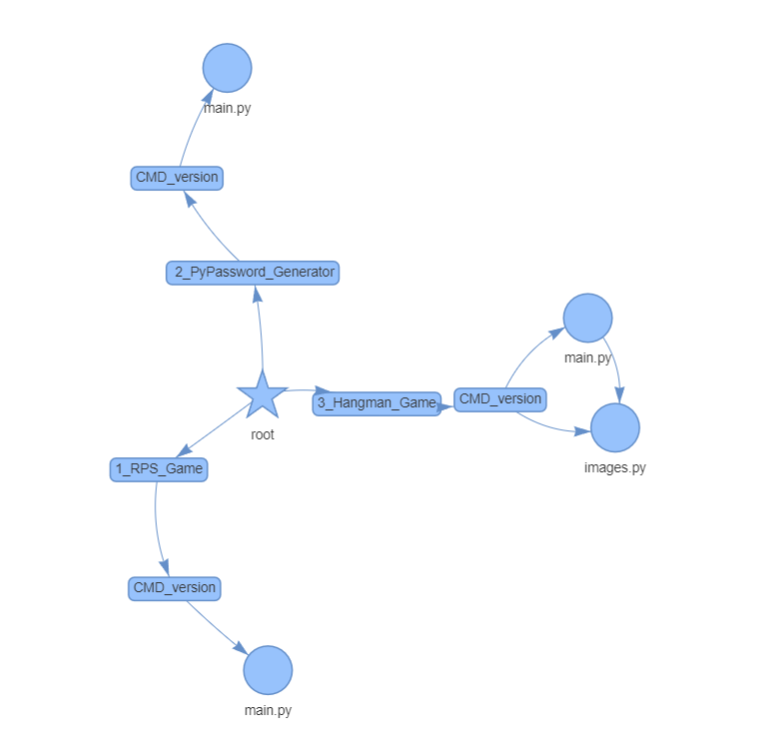
\includegraphics[width=0.5\textwidth]{graph.png}
    \caption{Voorbeeld van een graaf van de relaties tussen bestanden}
    \label{fig:graph}
\end{figure}

Er is een voorbeeld van een graaf te zien in \ref{fig:graph}, alsook is er een voor een groot project een graaf gemaakt om te kijken of de relaties tussen de bestanden duidelijk weergegeven worden op grote schaal \ref{fig:graph-large}.
De relaties op deze graaf zijn zichtbaar echter is het niet altijd duidelijk omdat er veel bestanden zijn en er bepaalde bestanden vaak geïmporteerd zijn.
Dit kan ervoor zorgen dat de graaf onoverzichtelijk wordt met de mate de grote van het projectOpenAi.

\begin{figure}[h]
    \centering
    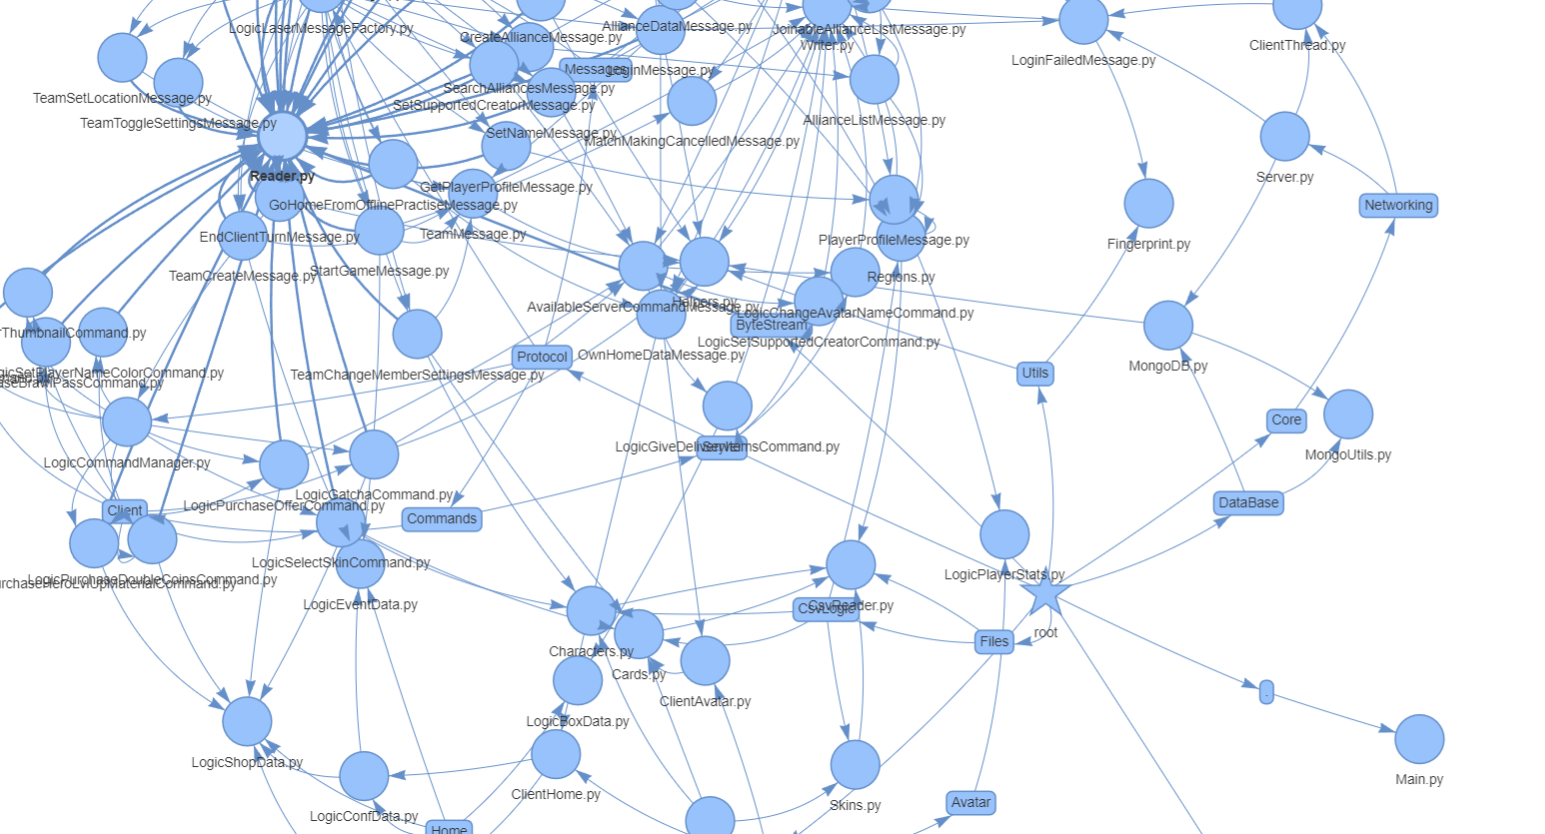
\includegraphics[width=1\textwidth]{graph-large.png}
    \caption{Voorbeeld van een fragment van een graaf van de relaties tussen bestanden van een groot project}
    \label{fig:graph-large}
\end{figure}